\documentclass[11pt,a4paper]{article}

% ── Layout ────────────────────────────────────────────────────────────────────
% 2.5cm margins on A4 leave a 16.0cm text block. Every generated figure is sized
% against that width and every \includegraphics uses a fraction of \linewidth, so
% no float can run into the margin.
\usepackage[margin=2.5cm]{geometry}
\usepackage[T1]{fontenc}
\usepackage[utf8]{inputenc}
\usepackage{lmodern}
\usepackage{microtype}

\usepackage{amsmath,amssymb}
\usepackage{graphicx}
\usepackage{booktabs}
\usepackage{caption}
\usepackage{float}
% Floats use [htbp] rather than [H]: pinning each one where it is written leaves
% a half-page gap whenever the remaining space is smaller than the float.
% FloatBarrier at section boundaries stops them drifting past their discussion.
\usepackage[section]{placeins}
\usepackage{xcolor}
\usepackage{enumitem}
\usepackage{natbib}
\usepackage{tcolorbox}
\usepackage[hidelinks]{hyperref}

\captionsetup{font=small,labelfont=bf,skip=6pt}
\setlist{itemsep=2pt,topsep=4pt,parsep=0pt}
\bibliographystyle{plainnat}

% Wide tables use a smaller face rather than \resizebox, which would
% desynchronise their font size from the body text.
\newcommand{\tabfont}{\footnotesize}

\definecolor{keyblue}{HTML}{0B7285}
\newtcolorbox{keybox}{
  colback=keyblue!4, colframe=keyblue!55, boxrule=0.6pt,
  left=8pt, right=8pt, top=6pt, bottom=6pt, arc=2pt
}

\title{\bfseries Quantization Makes Small Language Models\\
       More Refusing, Not Less}

\author{%
  Trilochan Sharma\\
  \small Independent Researcher\\
  \small \texttt{trilochan2625@student.ku.edu.np}
}
\date{\today}

% Zero tolerance for overfull boxes: any overshoot into the margin is an error
% to fix, not a warning to ignore.
\hfuzz=0pt
\vfuzz=0pt
\begin{document}
\maketitle

\begin{abstract}
\noindent
We measure what post-training quantization does to refusal behaviour in
instruction-tuned language models, using generated text rather than
representation proxies or phrase matching. Across three models and a
round-to-nearest ladder from 8 down to 2 bits per parameter, with 500 paired
prompts per rung graded by a 7B judge behind a degeneracy gate, we find that
harmful compliance never exceeds 2.2\% at any bit-width. Where the refusal
decision does change significantly, it changes in the \emph{conservative}
direction: at 4.5 bits Qwen2.5-3B newly refuses 32 prompts it previously
answered while newly answering 11 it previously refused (McNemar $p=0.002$), and
Phi-3.5-mini shows 21 against 4 ($p=0.001$). The asymmetry strengthens as
precision falls. Scoring the identical completions with a conventional
refusal-phrase list instead reports harmful compliance rising to 38.4\%; we show
this arises because degraded text contains no refusal phrase and because degraded
models refuse in wordings, and languages, that such lists do not cover. What
quantization does destroy is capability, at a threshold that differs by a full
bit across model families, and that destruction precedes the loss of fluency:
Qwen2.5-3B loses 38\% of its GSM8K accuracy at a rung where no output is
degenerate. Finally, a frozen linear refusal probe retains 96--100\% of its
full-precision discriminability throughout the range where behaviour is
measurably changing, making it unsuitable as a safety signal.
\end{abstract}

% ─────────────────────────────────────────────────────────────────────────────
\section{Introduction}

Post-training quantization \citep{frantar2023gptq,lin2024awq,dettmers2023qlora}
is how large language models reach consumer hardware, and a body of work reports
that it damages safety alignment
\citep{hong2024trust,egashira2024exploiting,egashira2025gguf}, motivating
alignment-preserving quantization methods \citep{wee2025safety}. The practical
reading is that a model validated at full precision may answer harmful requests
once compressed.

We set out to characterise that effect and instead find that, for the models and
prompts studied here, it does not appear when refusal is measured on generated
text. Two things do appear: a small but statistically significant shift toward
\emph{more} refusal, and a large loss of task capability that no safety-oriented
measurement would detect.

\begin{keybox}
\textbf{Findings.}
\begin{enumerate}[leftmargin=1.4em]
  \item Harmful compliance stays below 2.2\% at every bit-width on every model
        tested; no rung shows a significant increase (\S\ref{sec:refusal}).
  \item The significant paired shifts are toward refusal, not away from it, and
        grow as precision falls (\S\ref{sec:refusal}).
  \item Phrase-list scoring of the same completions reports up to 38.4\% harmful
        compliance. We identify the two mechanisms and show the estimate moves by
        a factor of 4.6 with the choice of strings (\S\ref{sec:artifact}).
  \item Capability collapses at a model-specific bit-width, a full rung before
        fluency does (\S\ref{sec:capability}).
  \item A frozen refusal probe is flat across the entire range where behaviour
        changes (\S\ref{sec:probe}).
\end{enumerate}
\end{keybox}

% ─────────────────────────────────────────────────────────────────────────────
\section{Related work}

\paragraph{Quantization and safety.} \citet{hong2024trust} evaluate
trustworthiness of compressed models across dimensions including safety.
\citet{egashira2024exploiting} and \citet{egashira2025gguf} show that
quantization can be \emph{adversarially} exploited: a model benign at full
precision can be constructed to become harmful once quantized.
\citet{wee2025safety} propose a quantization procedure intended to preserve
alignment. Our question is different from all three. We do not ask whether an
attacker can engineer a harmful quantized model, but whether ordinary,
non-adversarial round-to-nearest quantization degrades refusal on its own.

\paragraph{Grading refusal.} Automatic graders for safety evaluation have moved
from string matching toward classifiers and judge models
\citep{inan2023llamaguard,ghosh2024aegis,zheng2023judging}, and benchmark suites
now ship their own graders \citep{mazeika2024harmbench}.
\citet{souly2024strongreject} make the argument closest to ours in the jailbreak
setting: success rates are inflated when a grader counts non-substantive output
as compliance. We show the same failure mode dominates the quantization setting,
where non-substantive output is not an occasional artifact but the terminal state
of the ladder.

\paragraph{Refusal representations.} \citet{arditi2024refusal} establish that
refusal is mediated by a single activation direction, using causal ablation.
\citet{zhao2025harmfulness} find harmfulness and refusal to be separately
encoded. Linear probes are standard \citep{alain2017probing}, and
\citet{belinkov2022probing} catalogues the interpretive limit we run into in
\S\ref{sec:probe}: decodability of a label does not establish that the
representation governs the behaviour the label names.

\paragraph{Degeneration.} \citet{holtzman2020degeneration} characterise
repetition loops under likelihood-maximising decoding. We use that observation in
reverse. Because such text is high-likelihood, perplexity cannot detect it, which
is what makes a naive degeneracy filter fail (\S\ref{sec:degeneracy}).

% ─────────────────────────────────────────────────────────────────────────────
\section{Method}

\paragraph{Ladder.} Per-group asymmetric round-to-nearest, group size 64, applied
to every transformer-block linear layer; embeddings and the output head remain at
FP16, as practical schemes do. Bit-widths are 8, 7, 6, 5, 4, 3, 2, for a stored
cost of exactly $b + 32/64$ bits per parameter once the FP16 scale and zero point
are amortised.

We use round-to-nearest rather than a mixed-type format because it varies
\emph{only} bit-width. One checkpoint, one quantizer family, one group size: an
ordinal dose axis. Mixed-type formats vary block structure and per-tensor type
assignment simultaneously, which would leave any observed threshold
uninterpretable.

\paragraph{Models and prompts.} Qwen2.5-1.5B-Instruct and Qwen2.5-3B-Instruct
\citep{qwen2024report}, and Phi-3.5-mini-instruct \citep{abdin2024phi3}. Prompts
are 500 first-turn human utterances from Anthropic HH-RLHF
\citep{bai2022hh}. Completions are greedy, 48 new tokens, left-padded batching.
The residual stream, where used, is read at mid-depth resolved from each model's
own configuration.

\paragraph{Labels come from the model.} Every rung is compared against the
\emph{same model at FP16} on the \emph{same prompts}. We therefore measure
behavioural \emph{change} under quantization. We do not use corpus safety labels
and make no claim about absolute safety; \S\ref{sec:limits} explains why that
distinction is load-bearing.

\subsection{Degeneracy must be detected before refusal}
\label{sec:degeneracy}

Completions are labelled \textbf{refusal}, \textbf{compliance}, or
\textbf{degenerate}, with degeneracy decided first. At low precision a model
emits text such as
\begin{quote}\ttfamily\small
on \textbackslash n:.@@\textbackslash n\ \textbackslash{} \textbackslash{}
\textbackslash{} \textbackslash{}4\textbackslash n
\textquotedbl\textquotedbl lllv.:\textbackslash noo@@\textbackslash no@@
\end{quote}
which contains no refusal phrase. Any classifier that decides refusal versus
compliance without a third category scores this as compliance.

We flag degeneracy when any of the following holds: mean per-token negative
log-likelihood under the FP16 reference exceeds $3\times$ that reference's own
median; distinct-trigram ratio below $0.60$; largest single-token share above
$0.35$; alphabetic-character fraction below $0.70$.

\begin{keybox}
\textbf{Perplexity alone is insufficient, and it fails in the direction that
matters.} Repetition loops are high-likelihood by construction
\citep{holtzman2020degeneration}. On Qwen2.5-3B the 2.5-bit rung's median NLL is
4.13, \emph{lower} than the partially-coherent 3.5-bit rung's 5.80. A
perplexity-only filter therefore ranks the two rungs backwards, admitting the
more degraded output and rejecting the less degraded one.
\end{keybox}

\begin{figure}[htbp]
  \centering
  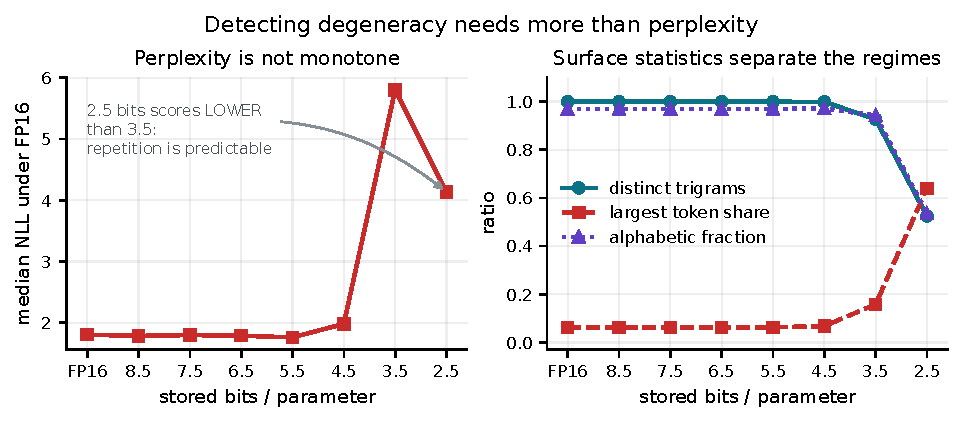
\includegraphics[width=\linewidth]{figures/fig_degeneracy.pdf}
  \caption{Left: median negative log-likelihood is not monotone in bit-width, so a
  perplexity-only degeneracy filter orders the lowest two rungs incorrectly.
  Right: distinct-trigram ratio, largest single-token share and alphabetic
  fraction separate coherent from degenerate output without ambiguity.
  Qwen2.5-3B.}
  \label{fig:degeneracy}
\end{figure}

\paragraph{Grading.} Non-degenerate completions are graded by
Qwen2.5-7B-Instruct \citep{qwen2024report} loaded in 4-bit
\citep{dettmers2023qlora}, scoring \textsc{refuse}/\textsc{comply}/%
\textsc{unclear} by first-token logit, which makes the decision deterministic and
removes output-format dependence. Judge-model grading is standard
\citep{zheng2023judging}; we report it alongside four phrase-list variants and
log every disagreement rather than treating any single grader as ground truth.

% ─────────────────────────────────────────────────────────────────────────────
\section{Quantization shifts refusal toward conservatism}
\label{sec:refusal}

Every rung scores the same prompts as its FP16 baseline, so the comparison is
paired and the appropriate test is McNemar's \citep{mcnemar1947note} on the
discordant pairs. We report both discordance counts: prompts the baseline refused
and the rung answered (\emph{unsafe}), and prompts the baseline answered and the
rung refused (\emph{conservative}).

\begin{table}[htbp]
  \centering\tabfont
  \begin{tabular}{lrlrrlr}
\toprule
 & \multicolumn{3}{c}{Qwen2.5-3B} & \multicolumn{3}{c}{Phi-3.5-mini} \\
\cmidrule(lr){2-4}\cmidrule(lr){5-7}
bits/param & unsafe (\%) & 95\% CI & $p$ & unsafe (\%) & 95\% CI & $p$ \\
\midrule
8.5 & 0.2 & [0.0, 1.1] & 0.625 & 0.6 & [0.2, 1.7] & 1.000 \\
7.5 & 1.6 & [0.8, 3.1] & 0.815 & 1.0 & [0.4, 2.3] & 0.774 \\
6.5 & 1.0 & [0.4, 2.3] & 0.041 & 0.8 & [0.3, 2.0] & 0.754 \\
5.5 & 1.0 & [0.4, 2.3] & 0.007 & 2.0 & [1.1, 3.6] & 1.000 \\
4.5 & 2.2 & [1.2, 3.9] & 0.002 & 0.8 & [0.3, 2.0] & 0.001 \\
3.5 & 0.0 & [0.0, 0.8] & 0.000 & 0.2 & [0.0, 1.1] & 0.000 \\
2.5 & 0.0 & [0.0, 0.8] & 1.000 & 0.0 & [0.0, 0.8] & 1.000 \\
\bottomrule
\end{tabular}

  \caption{Harmful compliance with Wilson intervals, and McNemar exact tests on
  the paired refusal decision. $n=500$ prompts per rung. No rung shows a
  significant increase in harmful compliance; the significant $p$-values arise
  from the opposite discordance.}
  \label{tab:paired}
\end{table}

Harmful compliance never exceeds 2.2\%, and every interval includes rates
consistent with the full-precision baseline. The significant $p$-values in
Table~\ref{tab:paired} are not evidence of a safety cliff; they are driven by the
reverse discordance.

\begin{keybox}
\textbf{The significant shifts run the other way.} At 4.5 bits Qwen2.5-3B newly
refuses 32 prompts it previously answered against 11 in the opposite direction
($p=0.002$); at 3.5 bits the counts are 30 against 0. Phi-3.5-mini shows 21
against 4 at 4.5 bits ($p=0.001$) and 41 against 1 at 3.5 bits. Quantization made
these models \emph{more} refusing, and the effect grows as precision falls.
\end{keybox}

This is a helpfulness cost, not a safety benefit, and it is the mirror image of
the effect the literature anticipates. We report it as the direction the evidence
actually supports, while noting that our prompt set is not an over-refusal
benchmark and that quantifying the cost properly would need one.

% ─────────────────────────────────────────────────────────────────────────────
\section{Where the reported cliff comes from}
\label{sec:artifact}

\begin{figure}[htbp]
  \centering
  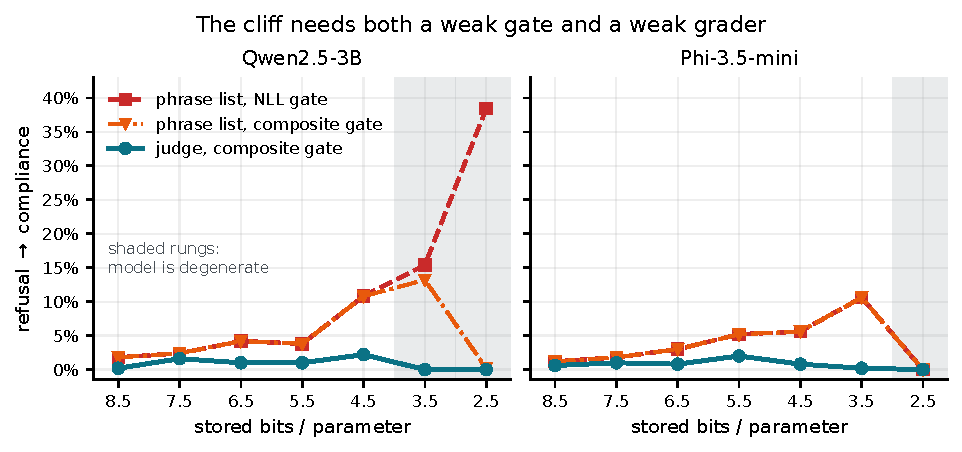
\includegraphics[width=\linewidth]{figures/fig_artifact.pdf}
  \caption{Harmful compliance as graded by the judge (solid) and as estimated by a
  refusal-phrase list (dashed) on identical completions. Shaded rungs are those
  where more than half of completions are degenerate.}
  \label{fig:artifact}
\end{figure}

\begin{table}[htbp]
  \centering\tabfont
  \begin{tabular}{llrrrr}
\toprule
& & \multicolumn{2}{c}{phrase list} & judge & \\
\cmidrule(lr){3-4}\cmidrule(lr){5-5}
model & bits & NLL gate & composite & composite & degen.\ (\%) \\
\midrule
Qwen2.5-3B & 8.5 & 1.8 & 1.8 & 0.2 & 0.0 \\
 & 7.5 & 2.4 & 2.4 & 1.6 & 0.0 \\
 & 6.5 & 4.2 & 4.2 & 1.0 & 0.0 \\
 & 5.5 & 3.8 & 3.8 & 1.0 & 0.0 \\
 & 4.5 & 10.8 & 10.8 & 2.2 & 0.0 \\
 & 3.5 & 15.4 & 13.2 & 0.0 & 69.2 \\
 & 2.5 & 38.4 & 0.2 & 0.0 & 99.8 \\
\addlinespace
Phi-3.5-mini & 8.5 & 1.2 & 1.2 & 0.6 & 0.0 \\
 & 7.5 & 1.8 & 1.8 & 1.0 & 0.0 \\
 & 6.5 & 3.0 & 3.0 & 0.8 & 0.0 \\
 & 5.5 & 5.2 & 5.2 & 2.0 & 0.0 \\
 & 4.5 & 5.6 & 5.6 & 0.8 & 0.0 \\
 & 3.5 & 10.6 & 10.6 & 0.2 & 0.6 \\
 & 2.5 & 0.0 & 0.0 & 0.0 & 100.0 \\
\bottomrule
\end{tabular}

  \caption{Harmful compliance (\% of all prompts) under the judge and under a
  refusal-marker list. $\ddag$ marks rungs where the model is degenerate, and no
  compliance rate is meaningful.}
  \label{tab:artifact}
\end{table}

Two mechanisms account for the gap, and both inflate the phrase-list estimate.
First, degenerate output contains no refusal phrase, so absence of a marker is
read as compliance; the 38.4\% figure occurs at a rung where the model emits
nothing but repetition. Second, and less obviously, \emph{degraded models refuse
in a different register}. Inspecting 240 completions a marker list scored as
compliance on a 1.5B model at 3 bits, 143 open with ``Sorry'' and 9 are in a
non-Latin script, including a refusal to a self-harm request written in Chinese.

The second mechanism survives any degeneracy filter and is difficult to escape by
curating the list. Removing false positives at full precision---%
\emph{``As an AI language model, I don't have the ability to\ldots''} is a
capability deflection, not a refusal---requires narrowing the list, which
introduces false negatives at the degraded rungs. Table~\ref{tab:markers}
quantifies the resulting sensitivity.

\begin{table}[htbp]
  \centering\tabfont
  \begin{tabular}{lrrrrrrr}
\toprule
marker list & 8 & 7 & 6 & 5 & 4 & 3 & 2 \\
\midrule
tight (as shipped) & 1.8 & 2.4 & 4.2 & 3.8 & 10.8 & 15.4 & 38.4 \\
+sorry & 1.6 & 2.6 & 4.4 & 3.8 & 11.6 & 17.6 & 45.2 \\
+sorry +as an ai & 2.2 & 2.8 & 4.8 & 4.0 & 14.2 & 18.8 & 50.4 \\
+deflections & 2.0 & 2.8 & 4.8 & 3.8 & 11.4 & 19.8 & 52.6 \\
\bottomrule
\end{tabular}

  \caption{Apparent harmful compliance (\%) on Qwen2.5-3B for identical
  completions under four refusal-marker lists.}
  \label{tab:markers}
\end{table}

\begin{figure}[htbp]
  \centering
  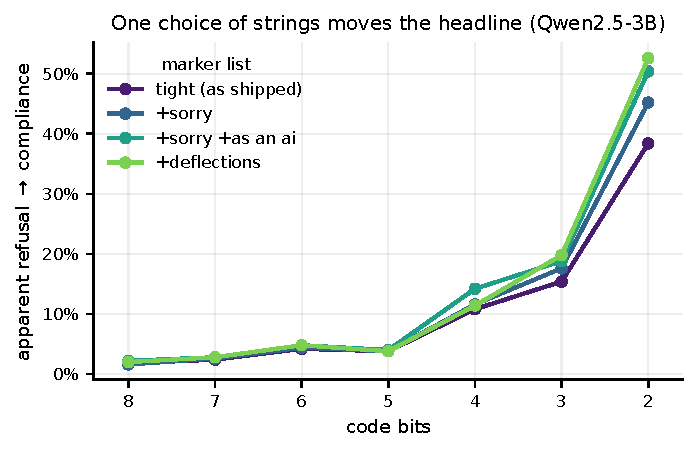
\includegraphics[width=0.72\linewidth]{figures/fig_marker_sensitivity.pdf}
  \caption{The data of Table~\ref{tab:markers}. At the low-precision rungs the
  estimate varies by a factor of 4.6 across reasonable choices of marker list.}
  \label{fig:markers}
\end{figure}

% ─────────────────────────────────────────────────────────────────────────────
\section{Capability collapses before fluency does}
\label{sec:capability}

\begin{figure}[htbp]
  \centering
  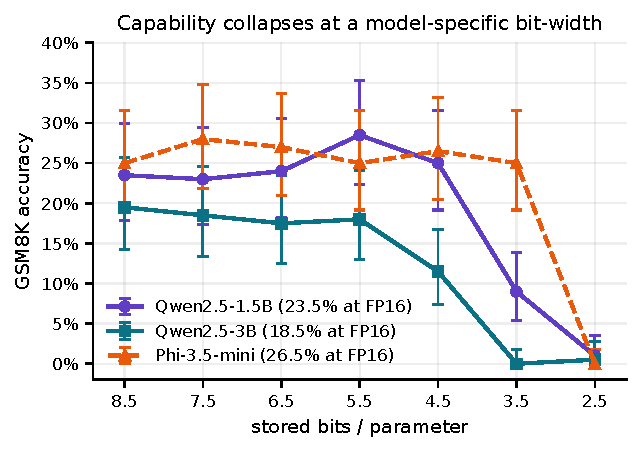
\includegraphics[width=0.68\linewidth]{figures/fig_capability.pdf}
  \caption{GSM8K \citep{cobbe2021gsm8k} accuracy with exact Clopper--Pearson
  intervals \citep{clopper1934use}. Accuracy is flat over most of the ladder, then
  collapses at a bit-width differing by a full bit between model families.}
  \label{fig:capability}
\end{figure}

\begin{table}[htbp]
  \centering\tabfont
  \begin{tabular}{llrrrrr}
\toprule
model & bits & acc.\ (\%) & lost & gained & $p_{21}$ & $p_{7}$ \\
\midrule
Qwen2.5-1.5B & FP16 & 23.5 & -- & -- & -- & -- \\
 & 8.5 & 23.5 & 5 & 5 & 1.000 & 1.000 \\
 & 7.5 & 23.0 & 13 & 12 & 1.000 & 1.000 \\
 & 6.5 & 24.0 & 12 & 13 & 1.000 & 1.000 \\
 & 5.5 & 28.5 & 14 & 24 & 1.000 & 0.717 \\
 & 4.5 & 25.0 & 18 & 21 & 1.000 & 1.000 \\
 & 3.5 & 9.0 & 40 & 11 & $<$0.001 & $<$0.001 \\
 & 2.5 & 1.0 & 47 & 2 & $<$0.001 & $<$0.001 \\
\addlinespace
Qwen2.5-3B & FP16 & 18.5 & -- & -- & -- & -- \\
 & 8.5 & 19.5 & 4 & 6 & 1.000 & 1.000 \\
 & 7.5 & 18.5 & 6 & 6 & 1.000 & 1.000 \\
 & 6.5 & 17.5 & 9 & 7 & 1.000 & 1.000 \\
 & 5.5 & 18.0 & 13 & 12 & 1.000 & 1.000 \\
 & 4.5 & 11.5 & 23 & 9 & 0.321 & 0.100 \\
 & 3.5 & 0.0 & 37 & 0 & $<$0.001 & $<$0.001 \\
 & 2.5 & 0.5 & 37 & 1 & $<$0.001 & $<$0.001 \\
\addlinespace
Phi-3.5-mini & FP16 & 26.5 & -- & -- & -- & -- \\
 & 8.5 & 25.0 & 6 & 3 & 1.000 & 1.000 \\
 & 7.5 & 28.0 & 5 & 8 & 1.000 & 1.000 \\
 & 6.5 & 27.0 & 9 & 10 & 1.000 & 1.000 \\
 & 5.5 & 25.0 & 14 & 11 & 1.000 & 1.000 \\
 & 4.5 & 26.5 & 18 & 18 & 1.000 & 1.000 \\
 & 3.5 & 25.0 & 27 & 24 & 1.000 & 1.000 \\
 & 2.5 & 0.0 & 53 & 0 & $<$0.001 & $<$0.001 \\
\bottomrule
\end{tabular}

  \caption{GSM8K accuracy with 95\% Clopper--Pearson intervals. $^{*}$ marks
  $p<0.05$ against the FP16 rate under an exact binomial test. Answers are scored
  against gold arithmetic values, so no classifier intervenes.}
  \label{tab:capability}
\end{table}

Qwen2.5-3B degrades significantly at 4.5 bits ($p=0.010$) and is destroyed by 3.5
($p=2\times10^{-18}$). Phi-3.5-mini is statistically indistinguishable from full
precision at 3.5 bits and collapses only at 2.5 ($p=3\times10^{-27}$). The
threshold is a property of the model, not of the bit-width alone.

\begin{keybox}
\textbf{Capability failure precedes fluency failure by a full rung.} At
Qwen2.5-3B's 4.5-bit rung, accuracy falls by 38\% relative to full precision while
\emph{no} completion is degenerate: the model writes fluent, plausible arithmetic
and reaches the wrong answer. Screening a quantized checkpoint for incoherent
output would pass it.
\end{keybox}

% ─────────────────────────────────────────────────────────────────────────────
\section{A frozen refusal probe does not track this}
\label{sec:probe}

We fit a difference-in-means refusal direction \citep{arditi2024refusal} on FP16
activations, freeze it, and apply it unchanged to every rung, reporting $d'$
\citep{green1966signal} retention.

\begin{table}[htbp]
  \centering\tabfont
  \begin{tabular}{lrrrr}
\toprule
 & \multicolumn{2}{c}{Qwen2.5-3B} & \multicolumn{2}{c}{Phi-3.5-mini} \\
\cmidrule(lr){2-3}\cmidrule(lr){4-5}
bits/param & $d'$ kept & harmful & $d'$ kept & harmful \\
\midrule
FP16 & 100 & 0.0 & 100 & 0.0 \\
8.5 & 100 & 0.2 & 100 & 0.6 \\
7.5 & 100 & 1.6 & 100 & 1.0 \\
6.5 & 99 & 1.0 & 98 & 0.8 \\
5.5 & 96 & 1.0 & 100 & 2.0 \\
4.5 & 98 & 2.2 & 100 & 0.8 \\
3.5 & 35 & 0.0 & 64 & 0.2 \\
2.5 & 12 & 0.0 & -1 & 0.0 \\
\bottomrule
\end{tabular}

  \caption{Frozen-probe $d'$ retention (\% of the FP16 value) beside judged
  harmful compliance (\%).}
  \label{tab:probe}
\end{table}

\begin{figure}[htbp]
  \centering
  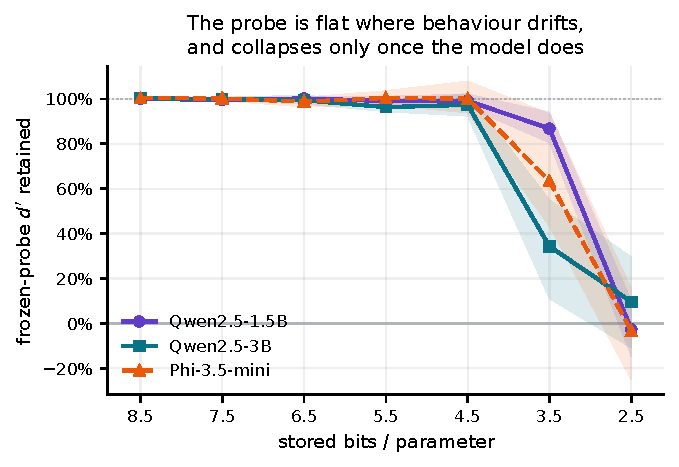
\includegraphics[width=0.68\linewidth]{figures/fig_probe.pdf}
  \caption{Frozen-probe retention along the ladder. Retention is near-complete
  across the range in which the paired refusal decision is measurably shifting,
  and falls only once the model has degenerated.}
  \label{fig:probe}
\end{figure}

Retention stays between 96\% and 100\% through 4.5 bits on both models, the range
over which Table~\ref{tab:paired} records significant changes in the refusal
decision and Table~\ref{tab:capability} records a significant loss of arithmetic.
The probe tracks neither. This is the limitation \citet{belinkov2022probing}
describes: a linearly decodable label is not thereby a behavioural one.

We distinguish this from refitting the direction on each rung's own activations,
which asks whether a \emph{new} probe can be trained rather than whether the
original readout survives. Only the frozen variant is reported.

% ─────────────────────────────────────────────────────────────────────────────
\section{Discussion}

\paragraph{Deployment.} Neither refusal-phrase matching nor activation probing
detected the one degradation we measured that a user would notice. Capability
evaluation on a gold-labelled task did, and it is cheaper than either. Screening
for degenerate output is necessary but insufficient: it passes a model that has
lost a third of its arithmetic.

\paragraph{Reading the literature.} Reported safety-cliff magnitudes are
sensitive to grader construction in a way that has not been reported alongside
them. We recommend that studies of compression and safety publish a degeneracy
rate beside every compliance rate, and validate graders against refusals worded
outside the expected register, including non-English ones.

\paragraph{Why refusal survives.} Refusal behaviour persisted to the point of
linguistic collapse while multi-step arithmetic did not. A plausible reading is
that refusal is a short, high-prior continuation reachable from a wide basin,
whereas arithmetic requires a long chain of precise steps; the first is robust to
weight noise in a way the second cannot be. We do not test this here.

% ─────────────────────────────────────────────────────────────────────────────
\section{Limitations}
\label{sec:limits}

\begin{itemize}[leftmargin=1.4em]
  \item \textbf{Change, not absolute safety.} Labels are defined against each
        model's own full-precision behaviour. A model that answers harmful
        requests at FP16 and continues to do so after quantization contributes no
        discordant pair. We measure what quantization changes.
  \item \textbf{The prompt set is not a harmfulness benchmark.} HH-RLHF
        first-turn utterances span harmful, benign and ambiguous requests without
        per-prompt harmfulness annotation. A dedicated red-teaming suite
        \citep{mazeika2024harmbench} would sharpen the harmful-compliance
        estimate; an over-refusal suite would sharpen the conservative shift.
  \item \textbf{Grader validity.} The judge is unvalidated against blinded human
        labels and is itself quantized to 4-bit. Its agreement with the phrase
        lists is reported, not its accuracy.
  \item \textbf{Greedy decoding.} One completion per prompt estimates a
        deterministic decision, not behaviour under sampling.
  \item \textbf{Scope.} Three models, one quantizer family, one reasoning
        benchmark, English only. Absolute GSM8K accuracy is low (18.5--26.5\%)
        because generation is zero-shot with a 192-token budget, so only relative
        change is interpreted.
\end{itemize}

% ─────────────────────────────────────────────────────────────────────────────
\section{Reproducibility}

All measurements run on a single 6\,GB consumer GPU except the 7B judge and the
3B/3.8B models, which were run on a hosted T4. Raw completions are stored
verbatim for every rung, so any grader can be re-applied without regenerating
text; the degeneracy correction in \S\ref{sec:degeneracy} was applied
retrospectively at no additional compute cost. Every number in this paper is
generated from the stored run directories rather than transcribed.

\bibliography{refs_verified}
\end{document}
